\chapter{Approche modulaire des réseaux de neurones}
\graphicspath{{01-Modularite/}}
\minitoc

%%%%%%%%%%%%%%%%%%%%%%%%%
% Intro du chapitre : Trouver un questionnement, un exemple qui parle de modularité dans les systèmes biologiques:  
% se placer dans le contexte de 
% - modularité : finalement on ne sait pas trop ce que c'est 
% - apprentissage ! 
% - réseaux de neurones
%%%%%%%%%%%%%%%%%%%%%%%%%

\section{Modularité}

\section{Mémoire associative et multi-modalité}
\draft{
\subsection{Mémoire associative}
Dans cette thèse, on s'intéresse à développer une mémoire associative via une architecture de cartes. La mémoire associative se définit par la capacité d'un réseau à apprendre des relations entre des ensembles de données et à pouvoir utiliser ces relations. Une tâche classique de mémoire associative sera la capacité de générer un motif en sortie à partir d'un autre motif d'entrée qui lui est associé, montrant que le réseau a appris la relation existant entre les deux éléments. 

\subsection{Multimodalité}
On parle de multimodalité lorsqu'on cherche à apprendre des relations entre données de différentes natures. Ce terme est souvent utilisé en robotique par exemple: les données issues de différents capteurs d'un robot sont les modalités. L'apprentissage multimodal cherche à apprendre ces modalités de façon commune. Ainsi, on peut effectuer un apprentissage multimodale en associant une modalité auditive consituée de signaux sonores et une modalité visuelle consituée d'images.
Un défi de l'apprentissage multimodal vient de la nature des signaux: comment faire pour que les modalités soient traitées de façon équilibrée ? 
%
}
\section{Cartes auto-organisatrices}\label{sec:som001}

Dans cette thèse, nous nous intéressons particulièrement aux architectures de \emph{cartes auto-organisatrices}, abrégées par SOM (Self-Organizing Maps). Le modèle de cartes auto-organisatrice a été initialement développé par Kohonen \cite{Kohonen1982}; le terme de cartes de Kohonen est ainsi utilisé pour désigner ce modèle initial. De nombreux modèles dérivés ont ensuite été développés à partir de ce modèle initial, sur diverses applications. On décompte par exemple plus de 11000 travaux utilisant les cartes de Kohonen dans la littérature en 2010(citer biblio).
Applications ?

Au sein de cette zoologie de cartes de Kohonen, nous passerons en revue dans ce chapitre deux familles de modèles de cartes auto-organisatrices dérivés des cartes de Kohonen: les cartes récurrentes traitant des données temporelles, et les modèles de cartes assemblées au sein d'une architecture.
\subsection{Carte de Kohonen classique}

Une carte de Kohonen est un algorithme de quantification vectorielle, cherchant à résumer un ensemble de données d'entrées issues d'un espace $\mathcal{D}$ en un nombre fini de vecteurs représentatifs, des prototypes.  Dans l'algorithme de Kohonen, ces prototypes sont disposés sur les noeuds d'un graphe, en général une grille en deux dimensions. Ce graphe est appelé carte de Kohonen. Les noeuds du graphe possèdent donc chacun un prototype et sont \emph{indexés}. Une distance entre noeuds est ainsi définie.
Au début de l'apprentissage, les prototypes ont une valeur aléatoires dans l'espace d'entrée. L'apprentissage est ensuite réalisé en trois étapes:
\begin{enumerate}
\item Une entrée $\inpx$ est présentée à la carte.
\item Le noeud ayant le prototype le plus proche de $\inpx$ selon une distance $d$, généralement la distance euclidienne, est choisie comme \emph{Best Matching Unit} (BMU) de la carte. Son index est notée $\bmu$.
\item Le prototype de la best matching unit est déplacé vers l'entrée $\inpx$, ainsi que les prototypes des noeuds voisins de $\bmu$ dans un rayon de voisinage défini à l'avance. On peut voir cette étape comme le déplacement d'une zone de la carte centrée en $\bmu$.
\end{enumerate}

L'algorithme de Kohonen repose donc sur à la fois un processus de compétition, avec la selection de la BMU de la carte, et un processus de coopération avec le déplacement des unités voisines de la Best Matching Unit et non seulement de cette dernière.
Toutes les données d'entrées sont tirées dans un même espace $\mathcal{D}$; par contre, la dimension de cet espace peut être quelconque.
L'apprentissage d'une carte de Kohonen se traduit par un rapprochement de tous les prototypes des données, de façon à ce que n'importe quel vecteur soit proche d'au moins un prototype. Visuellement, cela correspond à un dépliement de la carte dans l'espace d'entrée. On parlera donc de \emph{dépliement} d'une carte lorsque qu'on parle d'apprentissage. Ce dépliement est représenté en figures \ref{fig:som2d} et \ref{fig:som1d} pour des exemples de cartes en une et deux dimension, se dépliant sur des données en deux dimensions. 
A la fin de l'apprentissage, la carte conserve la structure topologique des données:
\begin{itemize}
\item Elle conserve les distances: deux prototypes ayant une distance proche dans la carte seront également proches selon la distance définie dans l'espace d'entrée. On observe donc une contiuité des valeurs des prototypes au sein de la carte
\item Elle conserve les densités. Une zone de $\mathcal{D}$ présentant plus de vecteurs aura plus d'unités la représentant dans la carte qu'une zone moins dense.
\end{itemize}
Par son aspect ordonné, une carte est une représentation en faible dimension d'un espace d'entrée de grande dimension. Les cartes de Kohonen sont ainsi utilisées dans de nombreuses applications, notamment pour visualiser des données de grande dimension et faire du regroupement de données (clustering). 

La carte de Kohonen est d'inspiration biologique. Le but premier de Kohonen était de développer un modèle informatique inspiré de l'organisation spatiale des neurones dans le cortex humain, dont un exemple est présenté en figure~\ref{fig:v1}. Il s'est notamment inspiré de l'organisation du cortex en colonnes corticales, ensemble de neurones réagissant à un même stimulus.

\draft{
(Kohonen book 1995)
In an attempt to implement a learning principle that would
work reliably in practice, effectively creating globally ordered maps of various
sensory features onto a layered neural network, this author formalized the
self-organizing process in 1981 and 1982 into an algorithmic form that is
now being called the Self-Organizing (Feature) Map (SOM) [2.27 -29J. In the
pure form, the SOM defines an "elastic net" of points (parameter, reference,
or codebook vectors) that are fitted to the input signal space to approximate
its density function in an ordered way. The main applications of the SOM
are thus in the visualization of complex data in a two-dimensional display,
and creation of abstractions like in many clustering techniques.

Motivations de Kohonen: capacité des régions du cerveau à s'auto organiser. Note que certes il doit y avoir un prédetermination génétique, mais qu'on observe une réorganisation des mapping lors de déficiences par ex. 

find abstract self-
organizing processes in which maps resembling the brain maps are formed,
whereas it is of less interest whether the maps are formed by evolution, post-
natal growth, or learning.

}

\begin{figure}
\centering
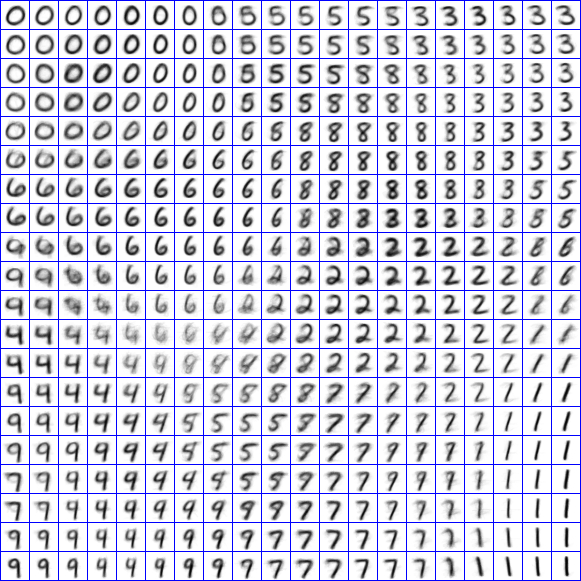
\includegraphics[width=0.5\textwidth]{digits.jpg}
\caption{Représentation de la base de données MNIST, images de chiffres écrits à main levées, par une SOM en deux dimension. Une continuité est observée dans la forme des images lorsqu'on se déplace dans la carte: le $0$ se transforme en $6$, etc.}
\label{fig:SOM}
\end{figure}



\subsection{Aspect topologique de la carte de Kohonen}

La carte de Kohonen se distingue d'autres algorithmes de quantification vectoriel par la topologie introduite par la carte dans l'ensemble des prototypes. Cette topologie dépend du voisinage utilisé par l'algorithme et de la dimension du support de la carte.
La plupart des algorithmes de SOM de la littérature utilisent comme support une grille en deux dimensions. L'indexation des noeuds est alors un ensemble de positions 2D.


En théorie, les cartes peuvent être une dimension (ligne), deux dimensions (grilles), ou de dimension plus grandes. Les cartes peuvent aussi être des graphes de forme plus variable. En pratique, les grilles deux dimension sont les plus couramment utilisées. Elles permettent d'effectuer une réduction de dimension, tout en étant facile à visualiser sur un écran. Les cartes de dimensions supérieures sont très rarement utilisées dans la littérature. Le cout de l'algorithme d'apprentissage dépend en effet du nombre de neurones, et celui-ci augmente exponentiellement lorsqu'on augmente la dimension d'une carte de Kohonen en plus de deux dimensions. Les calculs deviennent rapidement couteux, alors qu'un avantage de la carte de Kohonen est la simplicité et la rapidité de l'algorithme. Les cartes une dimension sont quant à elles limitées en terme de représentation des données, et sont donc rarement utilisées en pratique. Cependant, elles se prêtent bien à la représentation graphique. Nous utiliserons donc principalement des cartes en une dimension dans cette thèse.


De plus, les calculs et l'organisation générés par l'algorithme de Kohonen sont complexes déjà avec des cartes en une dimension. Leur description mathématique a été réalisée en \cite{cottrell_theoretical_2016,cottrell_theoretical_1998,fort_soms_2006}. La preuve de la convergence d'une carte a été réalisée seulement pour des cartes 1D et n'est pas généralisable directement au cas en deux dimensions. Les processus intervenant dans dans cartes 1D sont donc déjà mathématiquement difficiles à formaliser, difficulté qui augmente fortement avec les dimensions. Comme nous étudions dans cette thèse un nouveau modèle et cherchons à comprendre les mécanismes qui y interviennent, l'utilisation de cartes 1D réduit un peu la difficulté du problème. 
Les cartes de forme autre que 1D ou 2D sont moins couramment utilisées, mais peuvent avoir des avantages. On peut observer par exemple des cartes structurées en arbre \cite{koikkalainen_self-organizing_1990}, permettant une recherche de BMU structurée. Certains modèles construisent une carte de Kohonen noeud à noeud, donnant au final une carte de Kohonen sous forme d'un graphe construit par l'algorithme, telle que \cite{alahakoon_dynamic_2000}. 
\begin{figure}
\centering
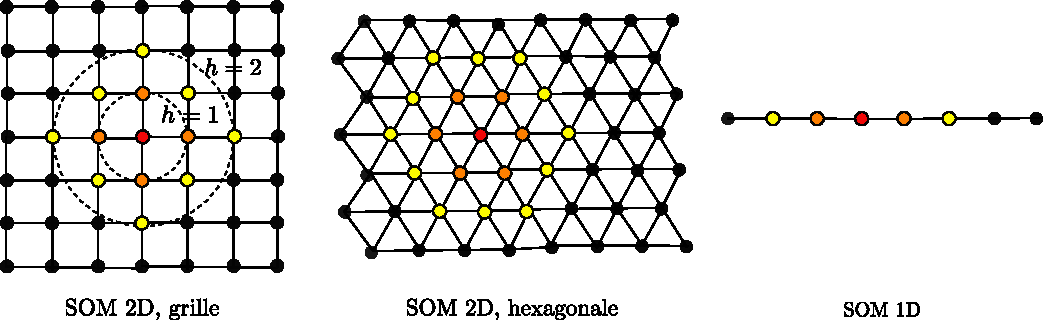
\includegraphics[width=0.8\textwidth]{soms_topologies}
\caption{Exemples de connexions dans le graphe support d'une SOM. Deux noeuds sont connectés s'il sont à une distance de une unité. Les SOM en deux dimensions sont les plus communément utilisées dans la littérature, sous forme d'une grille ou d'une grille hexagonale. Les SOM une dimension sont également utilisées.}
\label{fig:topo}
\end{figure}

\begin{figure}
\centering
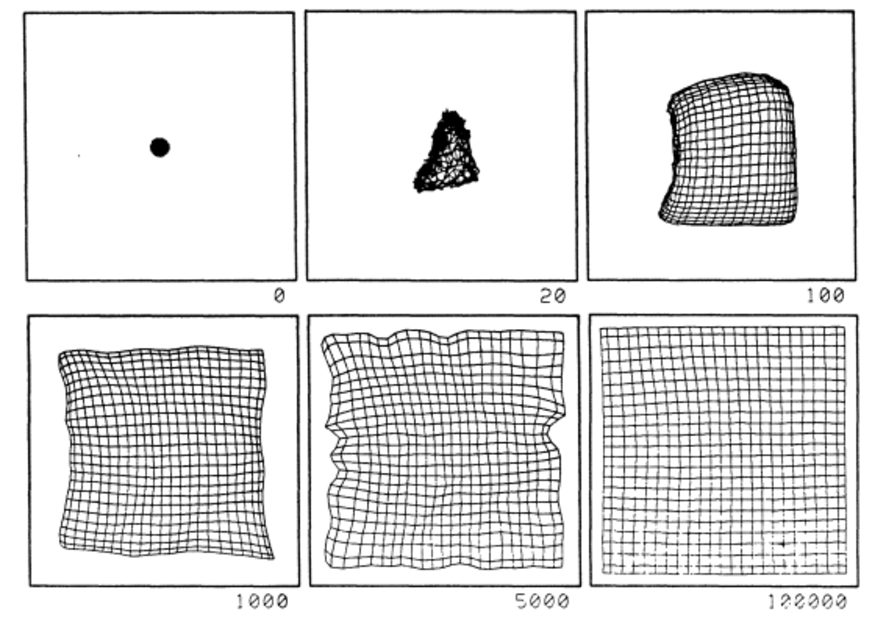
\includegraphics[width=0.7\textwidth]{som2d}
\caption{Dépliement d'une SOM 2D sur des données dans le plan $[0,1]^2$, \cite{Kohonen1995SelfOrganizingM} \label{fig:som2d}}

\end{figure}

\begin{figure}
\centering
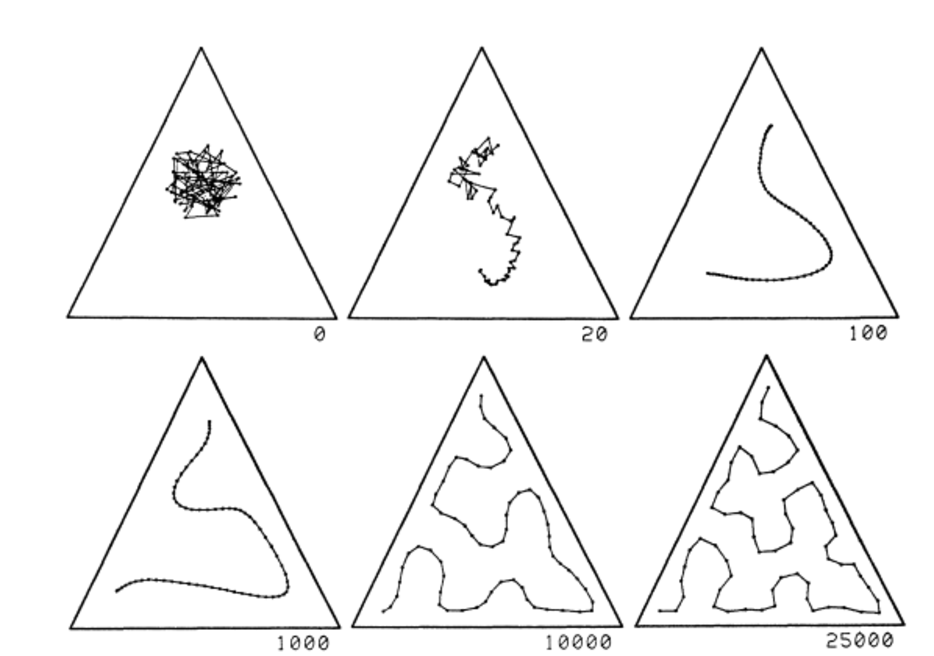
\includegraphics[width=0.7\textwidth]{som1d}
\caption{Dépliement d'une SOM 1D sur des données dans un triangle 2D \cite{Kohonen1995SelfOrganizingM}\label{fig:som1d}}

\end{figure}

\subsection{Inspiration Biologique d'une carte de Kohonen}

Le développement des cartes par Kohonen est intiallement inspiré par les cartes topologiques observées dans le cerveau. En effet, si on cartographie la position des neurones par rapport aux stimuli auxquels ils répondent dans certaines zones sensorielles du cerveau, on observe une disposition ordonnée. Les neurones proches réagissent à des stimuli proches. Un exemple est ainsi celui du cortex visuel v1, représenté en figure~\ref{fig:v1}. L'aire associée à l'audition présente aussi une organisation topographique (tonotopic maps), ainsi que de nombreuses autres aires, sensorielles ou plus abstraites [ref kohonen book].

\begin{figure}
\centering
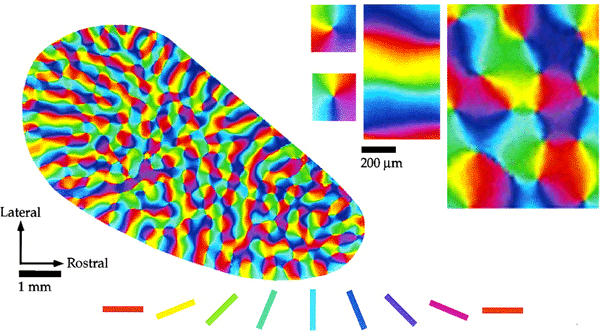
\includegraphics[width=0.6\textwidth]{v1.jpg}
\caption{Représentation des réponses du cortex visuel V1 à un stimulus visuel (batonnets d'orientation spatiale différentes). Les neurones répondant à une certaine orientation sont affichés de la même couleur. On observe une continuité entre les neurones proches dans le cortex et l'orientation à laquelle ils répondent. Cette propriété d'organisation est l'inspiration biologique des cartes de Kohonen. }
\label{fig:v1}
\end{figure}



\section{Motivations de la thèse : pourquoi construire une architecture de cartes auto-organisatrices modulaires}

\subsection{Inspiration biologique}
Nous avons vu d'un coté que les cartes auto-organisatrices sont d'inspiration biologique; sans chercher à modéliser les neurones du cerveau, on tend vers des principes généraux rappelant ce qu'on peut observer dans le cerveau. De la même façon, on observe dans le cerveau de multiples aires communiquant entre elles. Cette communication est observée en biologie lorsque des neurones d'une aire cérébrales activent des neurones d'une autre aire cérébrale. 
Ces connexions à l'échelle des aires cérébrales peuvent être rétroactives, c'est à dire que l'activation entre deux zones se fait dans les deux sens. Par exemple, \cite{primate_cortex_91}: zones dans le cortex du primate. La plupart des connexions est établie dans les deux sens.

La notion d'aire cérébrale renvoie à un aspect modulaire du cerveau. Modules préexistants mais flexibles: ainsi certaines zones qui s'avèrent non utilisées, suite par exemple à la perte d'un sens, se voient réorganisées au profit d'autre zones. On peut donc relier le cerveau à un modèle modulaire, avec des modules apprenant et pouvant se réorganiser.

Ainsi, de la même façon que les cartes auto-organisatrices rappellent l'organisation du cerveau sans chercher à le modéliser, l'architecture biologique observé dans le cerveau justifie l'idée de créer des architectures modulaires de cartes auto-organisatrices. Quitte à imiter la biologie, autant le faire jusqu'au bout.

On peut explorer plus en détail la notion de modules dans le cerveau. Des zones sont directement liées à des entrées externes, des zones sensorielles, de bas niveau. Le cerveau présente ensuite  d'autres aires liées à ces zones sensorielles, qui apportent de plus en plus d'abstraction dans les représentations des sens. Des aires sont aussi dédiées à l'assocation de plusieurs aires. On parle alors d'architecture hiérarchique, en référence à cette structure de zones sensorielles vers zones abstraites. Cependant, des connexions entre aires peuvent exister dans les deux sens. 

\draft{Le modèle de ces connexions n'est pas établi, mais plusieurs hypothèses et modèles existent en neurosciences computationnelles pour chercher à comprendre ce phénomène. Les plus répandues sont la zone de convergence divergence et la réentrée. A mettre dans modèle computationnels}

\subsection{Systèmes autonomes de cartes auto-organisatrices}

Un des enjeux de l'intelligence artificielle est de construire des systèmes autonomes, en robotique par exemple. Les cartes auto-organisatrices ont déjà comme avantage d'être un modèle d'apprentissage non-supervisé: l'ensemble des neurones et des poids réagit aux données présentées pour en dégager des représentations, sans intervention ou retour extérieur. Ensuite s'arrête l'aspect autonome: l'utilisation des cartes pour des tâches applicative nécessite une intervention extérieure. Il faut par exemple étiquetter les poids pour pouvoir faire de la classification d'entrées. La reconstruction d'image utilise la carte comme donnée pour faire du post processing de reconstruction. Utilisée comme algorithme de machine learning, la carte n'est pas un système autonome. 

Kohonen écrivait ainsi dans son livre à propos des enjeux des cartes de Kohonen en 1995:


\begin{quote}Systems of SOMs. A far-reaching goal in self-organization is to create
autonomous systems, the parts of which control each other and learn from
each other. Such control structures may be implemented by special SOMs;
the main problem thereby is the interface, especially automatic scaling of
interconnecting signals between the modules, and picking up relevant signals
to interfaces between modules. We shall leave this idea for future research. \cite{Kohonen1995SelfOrganizingM}
\end{quote}
L'idée d'un système de SOMs s'inscrit dans une recherche de système autonome. En introduisant des connexions entre cartes, on autorise le système à s'auto-activer au lieu de simplement réagir à des entrées, ce qui est nécessaire pour créer un système dynamique. Nous chercherons donc à créer un système de SOMs qui réagit à des entrées, mais qui peut ensuite s'auto-activer.

\subsection{Mémoire associative et SOM}

Les cartes auto-organisatrices sont utilisées pour faire de la mémoire associatives dans de nombreux travaux. 

%TODO : les lister :) 

L'implémentation d'une mémoire associative nécessite de fusionner des données de différent types en tant que modalités. Cette fusion peut être réalisée selon deux paradigmes:
\begin{itemize}
\item Les modalités sont fusionnées \emph{avant} leur présentation à l'algorithme. Il s'agit par exemple de présenter un vecteur concanténant deux modalités. Il s'agit d'une fusion au niveau des entrées.
%TODO exemples de fusions de ce type dans les cartes de Kohonen
Il faut faire attention à la façon dont les modalités sont assemblées: une peut prendre plus d'espace, être mieux prise en compte ...
\item Fusion de modalités au niveau de l'architecture. Dans ce cadre, l'idée est de garder des modules traitant les modalités séparemment, et l'apprentissage des liens entre les modalités est réalisé directement au sein de l'architecture. La signification de modalité est alors retranscrite dans l'architecture: la partie du réseau apprenant une modalité est uniquement associé à une modalité; son comportement pris séparément peut alors avoir un intérêt en lui-même à propos de la modalité considérée.
L'enjeu est alors de sélectionner les bons moyens de communication entre parties du modèle liées à chaque modalité.
\end{itemize}

Nous privilégions la deuxième option. Elle rejoint le cadre de systèmes autonomes et d'inspiration biologique; la parties du modèle renvoyant à une modalité précise est vue comme un module. Ces modules 


\subsection{Notion de mémoires}

De la même manière que les aires du cerveau, on observe différent types de mémoires interagissant dans un cerveau: mémoire épisodique, mémoire à long terme. Le temps et la mémoire est en quelque sorte spacialisé grâce aux échelles et aux temps de connexions dans le cerveau. 
La notion de mémoire se rapporte finalement aux architectures et systèmes autonomes. Les mêmes éléments de cerveau sont utilisés dans des cadre sensoriels et de mémoire. 
Des systèmes autonomes doivent présenter une mémoire. 
La notion temporelle a donc tout intéret à être intégrée à une architecture de cartes auto-organisatrices dans le cadre de rechercher des systèmes plus autonomes.

\subsection{Association de réseaux de neurones}

Parler du deep learning, des capacités d'émergence dans les systèmes complexes ?????

\subsection{Calcul décentralisé ? }

\section{Architectures de cartes auto-organisatrices}
Les cartes auto-organisatrices ont été largement étudiées depuis leur introduction en 1984. On dénombre de milliers de papiers en traitant, rien que sur la période 1984 - 2003 pour laquelle une bibliographie exhaustive par mot clés a été menée par Lampinen et Oja (ref). De nombreux papiers ont été publiés depuis, 10000 selon une recherche par mot clés sur google scholar. 

La question d'architecture de cartes de Kohonen a bien sur été explorée. Associer les cartes en modèle hiérarchique faisait même partie des premiers travaux publiés autour des cartes de Kohonen.
L'association de quelques cartes de Kohonen dans des applications spécifiques est également assez répandue:
(citer association de cartes pour détection d'erreur, autres applis ?). Tous ces modèles sont des constructions adaptées pour résoudre un problème de machine learning spécifique.

Mais étonnament peu de travaux, par rapport à la littérature sur le sujet, se sont intéressés à l'association de cartes en tant que nouveau modèle à part entière.

Dans cette section, nous passons en revues les modèles existantes permettant, d'une façon ou d'une autre, de connecter des cartes entre elle. Nous étudierons d'un coté les modèles d'architectures de plusieurs cartes communiquant via des interfaces; nous étudierons également les modèles de cartes récurrentes. Les cartes récurrentes sont appliquées à des motifs temporels et ont la caractéristique d'utiliser des éléments de leur état passé pour calculer leur état à un instant donné. La notion de communication est ici encore présente et peut nous servir d'inspiration pour développer une architecture de cartes. Par ailleurs, nous avons mentionné que le traitement de données temporel doit pouvoir être intégrée dans une architecture de carte visant à être autonome. Il s'agit ici de trouver une méthode d'interface entre carte qui puisse à la fois connecter des cartes auto-organisatrices et introduire des connections récurrentes dans le temps. 

\subsection{Modèles de neuroscience computationnelles}

De nombreux travaux de biologie observent des co-activations entre les zones du cerveaux. Le cortex cérébral est ainsi être considéré comme un reseaux de neurone modulaires, avec des régions s'activant entre elles. \cite{primate_cortex_91,mountcastle_columnar_1997,Harriger2012RichCO}

Ces coactivations aient été observées expérimentalement. Plusieurs modèles en neurosciences computationnelles ont été proposés pour expliquer ce phénomènes. Les modèles les plus communs sont la zone de convergence-divergence de Damasio (CDZ) \cite{damasio_time-locked_1989}, et le modèle de boucles de réentrées de Edelmann \cite{Edelman1982GroupSA}.

CDZ holds that specific cortical areas act as sets of pointers to other areas , and therefore connect several brain networks. The reentry theory hypothezise direct bidirectional exchanges between several brain areas. Those theories are a biological inspiration to create and connect modular networks.
L'étude des réseaux de neurones impulsionnels, utilisés notamment en neurosciences computationnelles, dégage des 
\cite{electronics9101605}

\subsection{Modèle de SOMs 1}
Contrairement aux réseaux impulsionnels qui utilisent des règles d'activation à l'échelle d'un neurone, les cartes auto-organisatrices (SOM) et de ses variantes (GSOM, Tree SOM) définissent des règles de calcul à l'échelle de la carte. Ces calculent s'appuient sur sur les distances et le voisinage, imitant les règles locales ; on parle donc de processus d'auto-organisation. Les motifs d'activation qu'ils développent sont alors similaires à ceux que l'on retrouve dans des zones cérébrales telles que le cortex visuel.
Il est donc pertinent d'étudier comment plusieurs cartes peuvent être connectées pour réaliser un calcul décentralisé.
De nombreux travaux utilisent des modèles incluant plusieurs cartes auto-organisatrices; mais la plupart de ces architectures sont conçues pour une application spécifique.
On ne peut donc pas parler de modèles modulaires. Certains travaux ont cependant développé des modèles modulaires conçus en combinant les cartes comme un nouveau modèle générique et exploiter les communications.

Dès que les SOMs ont été introduits, une version hiérarchique a été proposée, HSOM : \cite{lampinen_clustering_1992,koikkalainen_self-organizing_1990} . Dans HSOM, une carte apprend des données comme une première couche et transmet l'index de son BMU comme entrée à une deuxième carte. Les auteurs ont observé que la deuxième carte a une capacité de regroupement plus précise qu'une seule carte. Étonnamment, ce modèle n'est pas largement utilisé. Certaines variantes de HSOM ont été proposées par la suite, comme l'arbre d'architecture croissante soms [ref], où l'architecture hiérarchique est de plus en plus conçue pour s'adapter à l'ensemble des données. Dans ce cas, l'activité entière d'une carte est transmise en entrée aux couches supérieures. (Citons également [baruque])
Ces architectures hiérarchiques : commentaire
Dans \cite{dominey13}, les auteurs construisent des architectures hiérarchiques en transmettant les positions des BMU entre les cartes multimodales. L'inspiration est tirée du cadre CDZ.
D'autre part, certains travaux visent à connecter les cartes entre elles de manière directe, en se rapprochant de la théorie de la rentrée d'Edelman. C'est le cas de A-SOM : combiner des cartes.

Certains travaux développent des cartes modulaires où les connexions entre cartes sont créées neuronalement. C'est le cas de l'algorithme SOIMA \cite{SOIMA}, où les connexions entre neurones sont apprise avce une regle hebbienne alors que l'apprentissage se fait dans chaque carte : les neurones qui s'activent ensemble voient leur poids de connexion renforcé.

\section{Cartes auto-organisatrices récurrentes}

On appelle réseaux récurrents des réseaux de neurones qui prennent en compte leur état précédent pour calculer leur état actuel. Ces réseaux sont utilisés pour le traitement et l'apprentissage de signaux temporels. Citons par exemple, en deep learning, les RNN (recurrent neural networks), dont les neurones recoivent leur état précédent en entrée. Les réseaux récurrents les plus utilisés actuellement sont les LSTM, dans lesquel un système de portes perment d'activer ou non des neurones en fonction des états précédents du réseau. Les cartes de Kohonen ont elles aussi des version récurrentes que nous allons présenter dans cette partie.

Nous nous intéressons aux architectures multi-cartes, mais les cartes récurrentes répondent à des problèmes très similaire à ceux rencontrés dans la conception d'architectures de cartes pour faire de la mémoire associative. Dans une carte récurrente, le problème principal est de trouver comment communiquer à la carte de l'information sur son état précédent et comment utiliser cette information dans l'apprentissage de l'état courant. Cela rejoint la problématique posée dans les architectures de cartes de Kohonen, qui est de comment communiquer à une autre carte son état, afin de l'utiliser dans l'apprentissage de l'état courant. Nous avons vu précedemment qu'il existe assez peu de modèles d'architectures de cartes. Il existe plusieurs modèles de carte récurrentes qui nous permettrons de compléter cette étude. 

Notre volonté de créer un modèle général d'architecture de cartes auto-organisatrice motive également le fait de s'intéresser aux cartes récurrentes. On souhaite en effet créer un modèle qui puisse unir cartes récurrentes et cartes normales au sein d'une même architecture. L'aspect bio-inspiré du modèle et son aspect multimodal ciblent plutot des applications d'un tel réseau en robotique. Or, la plupart des données traitées par des réseaux de neurones, en particulier dans les applications robotiques, sont temporelles : vidéos, signaux sonores, capteurs de position. Il est donc important de s'appuyer autant sur les modèles de cartes récurrentes existantes que sur les architectures afin de créer un modèle général. 

%Enfin, les cartes de Kohonen ne se prêtent pas à un apprentissage en ligne de données en temps réel. En effet, il est nécessaires que les données d'entrées soient tirées aléatoirement dans l'espace à apprendre et ne suivent pas une trajectoire. Par exemple, si on veut apprendre des images, mais que les entrées sont données à la carte sous la forme d'une vidéo, les frames de la vidéo sont proches les unes des autres et forment donc une continuité dans l'espace d'entrée des images à apprendre. La carte va alors apprendre le sous ensemble de l'espace sur lequel se trouvent les premières frames, puis les oublier au fur et à mesure de l'apprentissage et les remplacer par les images qui suivent. Avec une architecture multi cartes qui prendrait en compte un aspect temporel, on pourrait imaginer la construction d'une architecture plus robuste.

Nous avons classé les modèles de cartes récurrentes existants en différentes catégories. D'une part, certains modèles de cartes utilisent l'état précédent de la carte lors du calcul de l'activité de l'état courant. De l'autre, des modèles réutilisent plutot des élement de la carte précedente en tant qu'entrée de l'état courant.

\subsection{Cartes récurrentes }

\draft{TKM, RSOM, utilisation seulement de la zone autour du BMU}

\subsection{Réutilisation d'élements en entrées}
%
%\section{Contexte}
%
%L'idée de ce chapitre est d'inscrire nos travaux dans le coté modulaire des réseaux de neurones. Il nous foudra donc définir proprement ce qu'on appelle modularité, et définir les motivations pour créer une architecture modulaire. Il faut def ce qu'on appelle réseau de neurones et apprentissage automatique. 
%
%D'une part, de nombreux modèles biologiques présentent des architectures modulaires. Notre conception du monde se présente en fait sous une forme de modularité. En tant qu'humain, nous comprenons le monde de notre point de vue, en le décomposant pour qu'il semble accessible : en effet notre raisonnement est modulaire, notre système social, groupes d'individus, etc, comme l'explique par exemple \cite{Morowitz1995TheMT} dans "How a mind resides in the brain".
%Nos contructions sont modulaires : programme informatique ... Il est difficile de concevoir et surtout de comprendre, en tant qu'humain, un système qui ne serait pas décomposable en modules. Prenons comme exemple les réseaux de neurones profonds : la compréhension  et l'interprétabilité ces programmes est un défi de la recherche actuelle. Pour cette interprétation, on cherche des éléments symboliques, des groupes, des communautés. 
%La décomposition des sciences elles même, par exemple, nous permet de trouver des solutions aux problèmes a des échelles différentes. Le programmeur n'a pas besoin de comprendre en profondeur quels transistors composent les circuits; l'expert.e en electronique n'a pas besoin de d'abord résoudre les équations qui régissent les mouvements ioniques au sein des transistors pour concevoir des circuits, etc. Seuls les principes régissant les comportement globaux d'un système commme le transistors ont besoins d'être connus pour utiliser ces sytèmes dans une tâche; tâche qui consituera également un module dans son ensemble et qui sera régie par des principes généraux, du transitor à l'utilisation d'un logiciel de dessin. 
%Mais est ce que cette hiérarchie modulaire est essentiellement subjective ? A priori non. Une organisation modulaire est présente et calculable dans de nombreux systèmes.
%
%
%Les modules sont également associés aux systèmes complexes. De nombreux travaux sont ainsi réalisés à la frontière entre domaines, 
%Réseaux associés aux systèmes complexes, interactions.
%
%
%\subsection{Systèmes complexes}
%
%Un système complexe se définit par un système présentant un grand nombre de composants interagissant de façon non-triviale, de façon non-linéaire, par exemple des rétroactions entre éléments. Ces systèmes présentent alors un comportement global qui semble impredictible par un raisonnement humain, même ayant l'information des règles locales qui régissent les interactions entre éléments. Le système ne peut alors s'étudier que par simulation ou étude de sa globalité, la compréhension indépendante de ses composants n'étant pas suffisante pour comprendre les mécanismes à l'oeuvre. C'est la théorie qu'on appelle holisme et qui se résumerait par : \emph{Le tout est plus que la somme des parties.}. Ce \emph{plus} signifie que des comportements émergent du système dans son ensemble, qui ne peuvent se décrire à des échelles plus petites. Un exemple de système complexe couramment présenté est le vol organisé d'oiseaux migrateur. Ces ensembles, parfois composés de milliers d'oiseaux, volent en groupe sans qu'il n'y ait une organisation avec un leader. Chaque oiseau possède une règle locale qui lui perment d'interagir avec ses voisins, qui peut se résumer par: 
%
%\begin{itemize}
%\item voler dans la même direction que ses voisins
%\item rester proche de ses voisins
%\item Ne pas entrer en collision
%\item Eviter les obstacles
%\end{itemize}
%
%Ces seules règles simples permettent, en simulation, d'observer un comportement de nuée. Ce vol groupé est alors le comportement \emph{émergent} du système : il n'est observable que globalement. Dans ce cas, un cerveau humain pourrait comprendre ce comportement. Mais ajoutons un peu de diversité au niveau des règles locales, et l'esprit est rapidement embrouillé. Ainsi, le jeu de la vie, un fameux automate cellulaire, est un système similaire aux nuées d'oiseaux . Dans cette simulation, des cellules sont disposées en grille, chacune ayant deux état possibles : "vivante" ou "morte". A chaque pas de simulation, les cellules mettent à jour son état en fonction de celui des 8 cellules alentours. Une cellule morte présentant exactement trois voisines vivantes nait, elle devient vivante. Une cellule vivante possédant deux ou trois voisines vivantes le reste. Une cellule vivante présentant moins de deux ou plus de trois voisines vivantes meurt (solitude ou étouffement). Ces règles locales sont incroyablement simples, mais en fonction des états initiaux, une multitude de comportements (motifs) voient le jour au cours de la simulation. Ces comportements ne peuvent être observés et compris qu'en simulant l'avancement du système.
%Ces comportement émergents présentent en particulier une forme d'organisation, comme les motifs des automates cellulaires. L'émergence d'une organisation est ainsi caractéristique d'un système complexe. 
%Globalement, tout système réel est complexe et résulte d'une interaction. Bien qu'on ait pu décomposer les comportements en sous-domaines, la complexité est partout dans la nature : les colonies de fourmis trouvent des chemins vers la nourriture via leurs interactions locales,
% 
%%Histoire de l'horloger et de la décomposition en modules/simu ?
%La quantification de la complexité d'un système est malgré tout une tâche compliquée à mettre en oeuvre. On a vu en effet qu'une des caractéristiques principales pour un système est l'appartition d'un comportement émergent. Mais, est-ce que
%
%%On ne peut pas parler de systèmes complexes sans parler de chaos. Le chaos est un mode de fonctionnement d'un système dynamique non-linéaire. 
%
%
%%Les systèmes, dans leur échelles, sont donc complexes. Si on peut décomposer des systèmes pour les étudier, ils restent liés au sein d'un vaste écosystème. Ainsi, l'étude de la modularité des systèmes est présente au sein des approches biologiques.
%%"Un système complexe est un ensemble constitué d'un grand nombre d'entités en interaction dont l'intégration permet d'achever une mission commune. L'étude de ce type de système ne peut passer que par la simulation.
%%Les systèmes complexes sont caractérisés par des propriétés émergentes qui n'existent qu'au niveau du système et ne peuvent pas être observées au niveau de ces constituants.
%%(wikipedia)". Ces constituants interagissent par des règles locales qui sont souvent simples, mais dont l'interaction forme des propriétés émergentes. Complexe ne veut pas dire que les relations et interactions sont difficiles a exprimer : un système est complexe du point de vue d'un observateur, mais les règles locales sont souvent simples. Des exemples de systèmes complexes sont ainsi le comportement de fourmis au sein d'une fourmilière, le comportement des oiseaux en nuée, les réseaux sociaux, l'interaction entre protéines, les réseaux de neurones biologiques dans le cerveau.
%%
%%L'Emergence de motifs et de phénomènes d'auto-organisation (turing patterns) \cite{turing52} sont même utilisés pour qualifier le système complexe. En 1952, Alan turing montre que dans un système chimique comprenant de la réaction entre éléments et de la diffusion, des motifs spatiaux émergent, a partir de conditions initiales presque uniforment. Ces motifs se retrouvent dans de nombreux systèmes, chimique ou non.
%%
%%Il n'y a a priori pas de définition commune concernant ce qu'on appelle un système complexe et comment le mesurer. On pourrait plutot voir la complexité comme une façon d'étudier un objet. Un exemple de définition de la complexité est celle de Kolmogorov, qui évalue la complexité par la taille du plus petit module permettant d'engendrer l'objet.
%
%
%%Qui dit système complexe dit système modulaire ?
%%Réseaux sociaux, communautés de fourmis, autant d'exemples montrant une emergence auto-organisée de modules. 
%
%
%\subsection{Auto-organisation et émergence}
%
%L'auto-organisation décrit les phénomènes d'apparence organisés qui résultent d'un processus d'évolution lié à des règles locales. L'auto-organisation apparaît donc dans des systèmes complexes, et plus précisément, apparaît toujours dans ces systèmes. Ces phénomènes auto-organisés sont des motifs spatio-temporels. Alan Turing montre par exemple qu’a partir d’un état presque uniforme de composants chimique, leur réaction et diffusion crée des motifs répétés~\cite{turing52}. Ces motifs sont créés a partir de règles locales, on est bien sur un phénomène auto-organisé. De façon surprenante, ces motifs appelés “turing patterns” sont présents dans de nombreux systèmes biologiques, par exemple sur la peau des animaux, voir figure~\ref{fig:turing_pattern}. On est ici sur des motifs spatiaux, observés pendant l'évolution d'un système. Les motifs auto-organisés peuvent aussi être spatio-temporels, c'est le cas des motifs émergeant des automates cellulaires, comme les planeurs, dont non seulement l'état à un instant de simulation est un motif récurrent, mais aussi la façon dont il évolue. Ces motifs spatio-temporels sont aussi observés dans l'activation électrique des neurones dans un réseau biologique ou simulé : les "spikes" émisent par les neurones forment des motifs récurrents, appris par les neurones. 
%
%\begin{figure}
%\begin{minipage}{0.5\textwidth}
%\centering
%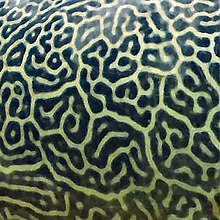
\includegraphics[width=0.6\textwidth]{220px-Giant_Pufferfish_skin_pattern_detail.jpg}
%\end{minipage}
%\begin{minipage}{0.5\textwidth}
%\centering
%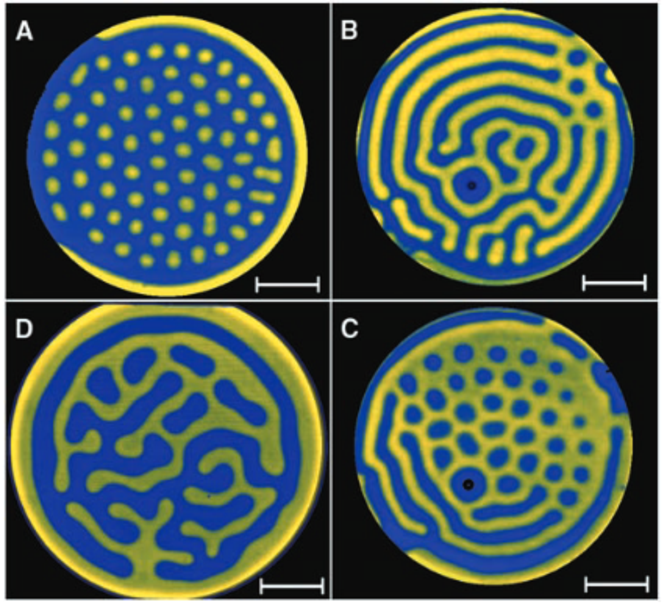
\includegraphics[width=0.7\textwidth]{turing_pattern_chem.pdf}
%\end{minipage}
%\caption{Motifs de turing sur la peau du poisson-globe, à gauche. A droite, motifs de turing émergeant d'une réaction chimique \cite{Horvth2009AnED}.}
%\label{fig:turing_pattern}
%\end{figure}
%
%\subsection{Apprentissage et systèmes complexes adaptatifs}
%
%Parmi les systèmes complexes, Holland et Gellman introduisent les Systèmes Complexes Adaptatifs~\cite{complex_adaptative_systemes}. Ces systèmes sont des systèmes complexes dont la particularité est, dans leur dynamique, de s'adapter à leur environnement. C'est précisément ce qu'on cherche à faire dans un réseau de neurones. On dira qu'il y a eu un apprentissage si l'évolution du système a conduit à l'émergence de propriétés montrant une généralisation d'information sur les données présentées. 
%
%\subsection{Questionnement du chapitre}
%
%Ce chapitre questionne l'intéret de s'inspirer de la biologie : 
%- pour développer une intelligence artificielle, et pourquoi on cherche a développer une intelligence artificielle, en fait ? 
%- mais aussi les intérets plus généraux d'étudier les réseaux biologiques, pour une meilleure compréhension des systèmes auto-organisés par exemple. 
%
%%%%%%%%%%%%%%%%%%%%%%%%%%%%%%%%%%%%%%%%%%%%%%%%%%%%%%%%%%%%%%%%%%%%%%%%%%%%%%
%% SECTION 1 : définitions et propriétés
%%- Tour d'horizons des définitions : en bio, en ingénieurie. Auto-organisation, conséquence de la modularité ? 
%%- Taxonomie : fonctionnelle, stucture modulaire,emergence 
%%- Position de l'autrice du manuscrit sur la modularité, intéret des différentes modularités
%%- Discussion : est ce que notre esprit modulaire veut trouver de la modularité a tout prix ? ( quand la mod est fonctionnelle, peut etre biais de nos représentations ? Mais, on observe assez objectivement des modules physiques via les connexions dans de nombreux réseaux. Evolution l'a fait comme ca, probablement une réponse globale a un problème. 
%%- Echelles de la modularité. 
%%- Activation d'autres modules
%%- Mutli-modalité - un mot, rappel dans une autre partie
%%%%%%%%%%%%%%%%%%%%%%%%%%%%%%%%%%%%%%%%%%%%%%%%%%%%%%%%%%%%%%%%%%%%%%%%%%%%%%%%
%
%\section{Quelle définition de la modularité ?}
%
%L'étude de la modularité des systèmes est vaste. Entre étude des systèmes biologiques, ingénieurie des réseaux de neurones, ou même sociologie, les définitions de modularité varient. Nous chercherons donc dans cette partie à exhiber des définitions et des spécificités de ce qu'on appelle modularité.
%
%\subsection{Modularité structurelle}
%
%Lorsque le système possède une structure définie de réseau, typiquement un réseau de neurones, on peut définir une modularité en terme de graphe. Un système modulaire est ainsi \emph{Un système qui a une structure de graphe modulaire}.
%Même en tant que graphe, modulaire est un terme large. 
%%De nombreux travaux proposent "une architecture modulaire" sans vraiement définir ce terme. 
%
%\subsubsection{Mesurer la modularité structurelle d'un réseau}
%
%La modularité d'un réseau est définie en théorie des graphes par le fait de pouvoir détecter des zones fortement connectées au sein de ce réseau, reliées par peu de connexions. Il s'agit donc de détecter des cliques, des sous-graphes fortement connectés, et de les différencier des zones moins connectées. 
%La quantité la plus largement utilisée pour définir la	modularité d'un graphe est le \emph{coefficient de clustering}. Ce coefficient mesure la probabilité que deux noeuds soient directement connectés en sachant qu'ils ont un voisin en commun. Les réseaux sociaux par exemple, présentent des forts coefficients de clustering. D'autres mesures sont possibles, menant à une détection de zones fortement connectées. Cette modularité peut également se mesurer en regardant la densité des arêtes dans une partition du graphe, relativement à ce qu'on attendrait dans un graphe aléatoire. 
%
%%\cite{Harriger2012RichCO}-> mesure modularité dans le cerveau, partie "méthodes" explique les méthodes de mesure de modularité. TODO les lister
%
%\subsubsection{Réseaux en "petit-monde"}
%
%La modularité d'un réseau est reliée à la propriété de petit-monde d'un graphe. 
%Un graphe en \emph{petit-monde} (small-world network) est un graphe dans lequel la distance moyenne entre deux noeuds est proportionnelle à $\log(N)$, $N$ étant le nombre de noeuds du graphe. En d'autres termes, c'est un graphe dans lequel on trouvera forcément un chemin assez court relativement à la taille du réseau, entre n'importe quels noeuds. Un exemple typique de réseau en petit monde est celui des relations sociales avec la règle des "six degrés de séparation" mis en lumière par Stanley Milgram en 1967 \cite{Milgram1967TheSW} : en prenant deux individus au hasard aux états unis, Milgram montre qu'on peut les relier de connaissance mutuelle en connaissance mutuelle en, en moynenne, 6 étapes. Maintenant que la plupart de nos connaissances sont en enregistrées sur les réseaux sociaux, cette distance, entre tous les utilisateurs de facebook dans le monde entier, a été mesurée comme étant 3.5 degrés de séparation en 2016 \footnote{\url{https://research.fb.com/three-and-a-half-degrees-of-separation}}. La propriété de petit-monde est mesurée par le \emph{coefficient de petit-monde} $\sigma$. Il se mesure en comparant des métriques du graphe avec celles d'un graphe aléatoire équivalent, c'est à dire un graphe aléatoire ayant le même nombre de noeuds et la même densité de connexions. 
%En notant $C$ le coefficient de clustering du graphe, $C_r$ celui d'un graphe aléatoire équivalent, $L$ la longueur (nombre d'arête) moyenne du plus court chemin entre tous les noeuds du graphe, et $L_r$ cette longueur dans un graphe aléatoire équivalent. 
%
%$$\sigma = \frac{\frac{C}{C_r}}{\frac{L}{L_r}} $$
%
%Un réseau est dit petit-monde si $\sigma > 1$, autrement dit, si la longeur du plus court chemin est inférieure à celle d'un graphe aléatoire, et/ou si le graphe présente plus de communautés qu'un graphe aléatoire. Cette métrique est cependant assez limitée, et il est plus judicieux existe d'autres mesures, comparant cette fois le coefficient de clustering et la longeur moyenne du plus court chemin à des graphes équivalents en treillis en plus des graphes aléatoires. 
%
%Un réseau petit-monde n'est pas forcément modulaire. Par contre, un graphe ayant une structure modulaire, avec des communautés fortement connectées, est petit-monde. Un exemple est donné en figure~\ref{fig:graphe}. Le réseau $(b)$ est petit-monde : on trouve forcément un chemin court entre deux noeuds. Le réseau $(c)$ est également petit-monde, mais présente aussi des sous-graphes fortement connectés. 
%La propriété de petit-monde semble avoir des avantages computationnel et se retrouve ainsi dans de nombreux exemples de réseaux biologiques. Nous détaillerons cet avantage en partie suivante. 
%
%\begin{figure}
%\centering
%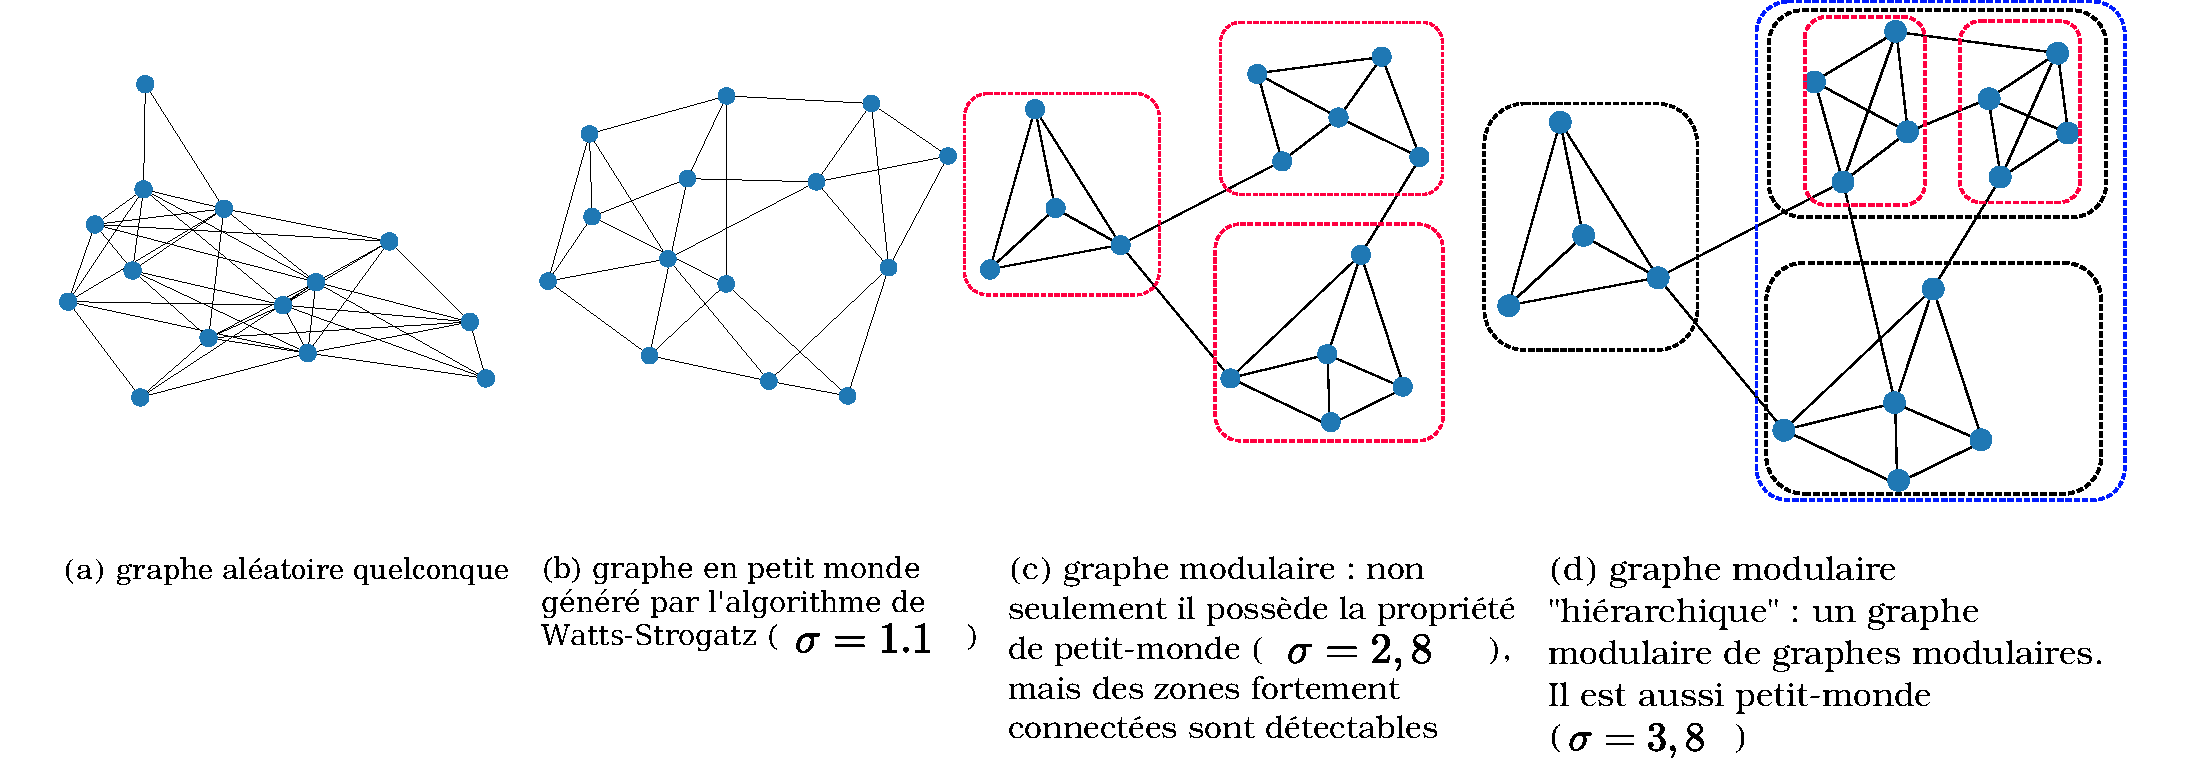
\includegraphics[width=\textwidth]{types_graphes.pdf}
%\label{fig:graphe}
%\caption{Exemples de graphes $(a)$ aléatoire, $(b)$ en petit monde, $(c)$ modulaire et $(d)$ modulaire hiérarchique.}
%\end{figure}
%
%
%\subsubsection{Modularité auto-similaire}
%
%Si on prend un sous-graphe fortement connecté d'un graphe modulaire, ce sous-graphe peut éventuellement, à son tour, présenter une structure modulaire. On peut alors parler de modularité \emph{hiérarchique}, ou \emph{auto-similaire}. L'auto-similarité renvoie au processus de construction dans lequel on connecte par une arête deux structures jumelles (par exemple deux graphes complets); on copie ce graphe et on le connecte par une arête à sa copie pour former un graphe plus grand, etc. On gardera le terme auto-similaire pour parler de graphes formés de modules de modules, même si ces modules ne sont pas des copies exactes d'eux mêmes à différentes échelles, afin de garder le terme hiérarchique pour d'autre structures. Cette modularité "à différentes échelles" est souvent présente dans les réseaux. Le cerveau est par exemple souvent présenté comme un réseau modulaire auto-similaire \cite{Meunier2010ModularAH}. Des modules larges (aires fonctionnelles) sont formés de sous-modules, eux mêmes décomposables en sous-modules, etc. 
%
%\subsubsection{Réseaux invariant par échelle}
%
%Un dernier type de réseau à relier à la modularité sont les réseaux sans échelles (\emph{scale-free networks}). Un réseau small world est un réseau dont le nombre de noeuds de degré $k$ suit une loi de puissance. Les réseaux sans échelles ont notamment été étudiés par Barabasi lors de l'étude du world wide web, \cite{Barabasi2003ScaleFreeN}.
%Ces réseaux sont "ultra-modulaires", ils ont un coefficient de clustering élevé. Il se caractérisent par la présence de sous-graphes ultra-connectés par des \emph{hub}, un noeud qui connecte d'autres noeuds moins connectés. Par leur distribution de connexions, on retrouve également dans ces réseaux une propriété d'auto-similarité: un sous-graphe autour d'un hub présentera une structure similaire à un sous-graphe plus grand, centré sur un plus gros hub, les hubs étant reliés entre eux. Par cette modularité, ils présentent donc aussi une caractéristique de petit-monde. Ces réseaux sont répandus au sein des structures sociales, par exemple les réseaux de citations entre articles scientifiques, les réseaux sociaux.
%
%\subsubsection{Conclusion}
%
%Un réseau dit "modulaire" exhibe donc souvent d'autres topologies plus spécifiques, telles que la propriété de petit-monde ou de réseau invariant d'échelle. Ces topologies sont détectées par différentes métriques s'appuyant sur les connexions sur réseau. Ces topologies se recoupent, un réseau modulaire étant généralement petit-monde, et un réseau invariant d'échelle ou modulaire hiérarchique étant modulaire. 
%La modularité et ces topologies induisent des propriétés particulières dans les dynamiques de graphe, décrites en partie suivante. Les réseaux existant réellement, tels que les réseaux de neurones biologique, les réseaux sociaux, semblent partager ces structures très spécifiques que sont la modularité hiérarchique et l'invariance d'échelle \cite{Harriger2012RichCO, Meunier2010ModularAH, Clauset2008HierarchicalSA, Ravasz2002HierarchicalOO}. Ces structures sont donc génériques dans la nature. 
%
%\subsection{Modularité fonctionnelle}
%
%Nous avons vu que des réseaux peuvent être définis de modulaires dans la partie précédente ; cette décomposition, cependant, n'est pas forcément unique et directe. 
%Définition des système complexe selon Le Moigne : le système dépend de la question que l'on cherche a étudier. Le système est complexe, mais sa décomposition et son analyse dépendra complètement de la question. Il n'y aurait donc pas un système intrinsèquement modulaire mais une approche adaptée au problème qui permet une décomposition. JL Le Moigne, La modélisation des systèmes complexes. 
%Selon lui, le système est complexe d'un point de vue de l'observateur, car les comportements qui agissent au sein du système semblent imprévisibles; par contre, on peut le décomposer pour le comprendre. 
%Donc si on veut étudier un système "réel", sa modularité dépend en fait de ce qu'on veut étudier. 
%Edgar Morin pensée complexe (?)
%
%Différence structure/organisation -> A mettre dans modularité ?? 
%
%
%Conclusion de la sous-section : la modularité d'un système complexe n'est pas forcément unique. Elle dépend de ce qu'on cherche à simuler ou étudier. Dans notre cas, on construira un système a partir de modules, on a donc une modularité directement définissable. Il semble cependant nécessaire de savoir la question que l'on cherche a étudier en définissant cette modularité. 
%
%%\subsection{Modularité temporelle}
%%
%%Du point de vue du système dynamique, l'aspect temporel n'est finalement qu'une dimension de plus dans la modularité du système. Les règles locales faisant évoluer le système dynamique amènent à des comportements complexes temporellement parlant. Par exemple, un attracteur fractal est le résultat des trajectoires d'un système dynamique complexe à l'état de chaos. 
%%
%%La modularité s'associe aux séquences dans le cerveau. Les mémoires, l'interaction entre échelles de fonctionnement apportent une modularité supplémentaire.
%
%\subsection{Emergence d'une modularité et auto-organisation}
%
%Dynamique des systèmes complexes : évolution qui mène à un système complexe ???
%
%
%% SECTION 2 introduction via la biologie, exemples 
%%%%%%%%%%%%%%%%%%%%%%%%%%%%%%%%%%%%%%%%%%%%%%%%%%%%%%%%%%%%%%%%%%%%%%%%%%%%%
%
%\section{La modularité, répandue dans les système biologiques}
%
%% Passer cette partie après la section définition ???
%\subsection{Le cerveau, réseau modulaire fondamental}
%
%Un neurone est un système dynamique, donc l’activité electrique est régie par des équation d’évolution dépendant des connexions qu’il recoit. Le cerveau dans son ensemble est alors,  fondamentalement, un agrégat de neurones. 300 neurones dans le ver microscopique  Caenorhabditis elegans, un million dans le cerveau des insectes, jusqu’a 86 millards de neurones dans un cerveau humain. Tous ces pics electriques et chimiques nous permettent une prise de décision, une mémoire, de la réflexion, des représentations …. Un ensemble de capacités que l’on nomme intelligence. Cette intelligence n’est pas localisée à un endroit précis dans le cerveau, de ce qu’on sait. Elle résulte de l’activité globale de l’ensemble de neurones, et est ainsi une propriété émergente. 
%
%Cet amas est le point de départ des études autour de l’intelligence artificielle. Si on veut créer un systèmes ayant une intelligence émergente, il nous faut comprendre les mécanismes de cette émergence, et donc comprendre les systèmes existant ayant cette capacité. Les réseaux de neurones se sont donc d’abord inspirés du cerveau avant d’être développés plutot sur un aspect computationnel avec moins de vraisemblance biologique.
%Cette inspiration biologique ne se limite pas à assembler des neurones : l’architecture cérébrale à plus grande échelle est aussi une source d’inspiration dans la recherche de systèmes intelligents, autrement dite, intelligence artificielle.  
%Et le cerveau semble avoir une architecture particulière : il est modulaire, à plusieurs échelles. 
%Les premières propositions de modèle du cerveau humain datent du début du XXeme siècle. Déjà, un découpage en aires est proposé pour expliquer le fonctionnement de cet organe, notamment avec les travaux de Broca et Wernicke qui mettent en lumière des zones du cerveau qui semblent responsable du langage. Le modèle connexioniste du cerveau, formalisé à partir de ces travaux par Geschwind dans les années 60 , décompose ainsi le langage en plusieurs fonctions : la compréhension, la lecture et l'action de parler. Ce modèle n'est plus vraiment utilisé, mais l'idée de décomposition en modules reste valable.
%Avec l'avènement des outils d'imagerie, le cerveau a pu être cartographié plus préciséement en un ensemble d'aires, agissant comme modules fonctionnels au sein d'une structure complexe; ces aires sont elles mêmes composées de modules distincts. 
%
%L'étude des aires et des connexions entre zones du cerveau, comme~\cite{primate_cortex_91} dans le cas du cortex visuel du primate, découpent les zones activée pour la vision en modules distincts, et montrent que ces modules sont connectés. Ces connexions, en fonction des modules, sont réciproques ou non. Les "pathsways" du cerveau désignent des modules fortement connectés. Leur détection expérimentale est réalisée en relevant des indicateurs de dépendance (corrélation, ..., en fonction des méthodes utilisées). Ainsi, \cite{Rolls2002ComputationalNO} précise la structure des différentes aires cérébrales en présentant les connexions au sein de ces aires, par exemple la structure présentée en figure~\ref{fig:cortex2} pour l'aire visuelle. 
%Les connexions du cerveau sont présentes à différentes échelles: des pathsways existent ainsi au sein de l'aire visuelle du cerveau, mais des boucles de rétroaction entre zones cérébrales sont présentes à plus grande échelle, par exemple la boucle baso-thalamo-corticale. Ces différentes échelles au sein du cerveau amènent \cite{Meunier2010ModularAH} à le présenter comme un réseau "hiérarchique modulaire". Cette activité "sans échelle" pourrait notemment permettre au cerveau d'appréhender les notions temporelles, transposant ainsi un réseau spatial en une activité temporelle \cite{biyu_scale-free_2014}.
%
%La structure cérébrale est donc bien particulière. Aussi, l'inspiration cérébrale des modèles d'intelligence articielle ne se résume pas au modèle neuronal, les éléments architecturaux et de connexions sont donc à considérer. 
%\begin{figure}[t]
%\centering
%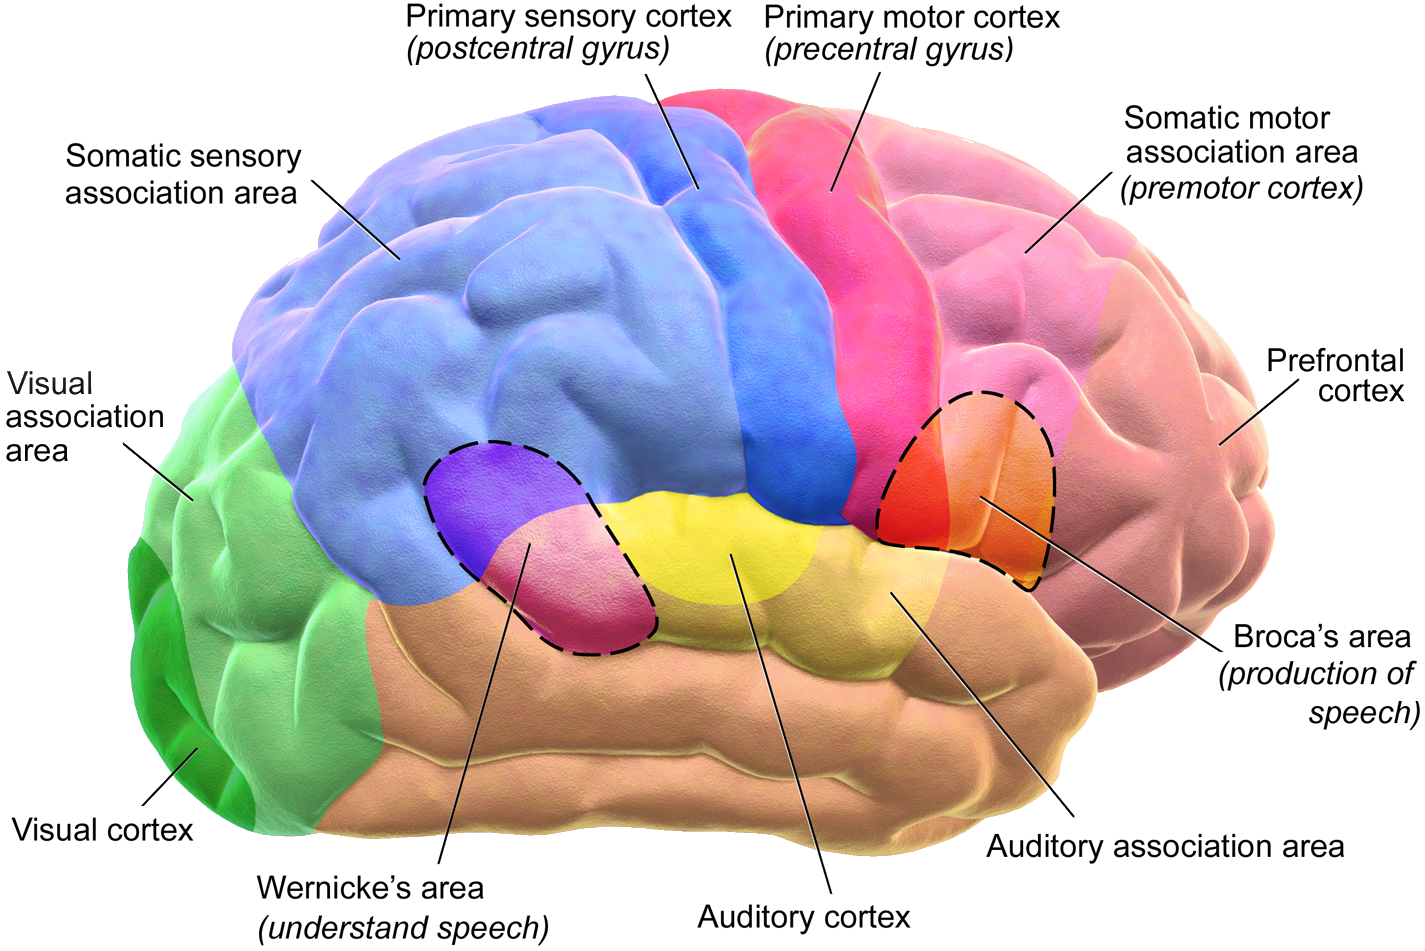
\includegraphics[width=0.5\textwidth]{Blausen_0102.png}
%\caption{Aires du cerveau humain}
%\end{figure}
%
%\begin{figure}[t]
%\begin{minipage}{0.5\textwidth}
%\centering
%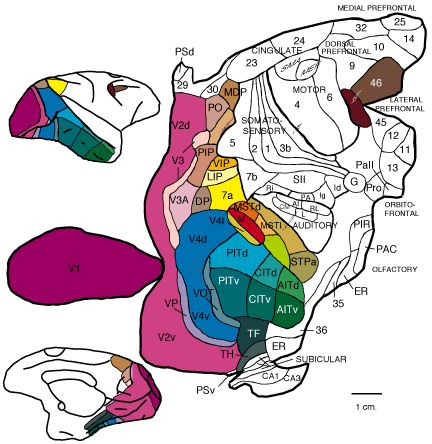
\includegraphics[width=0.7\textwidth]{FVE_fig2map.png}
%\label{fig:cortex1}
%\end{minipage}
%\begin{minipage}{0.5\textwidth}
%\centering
%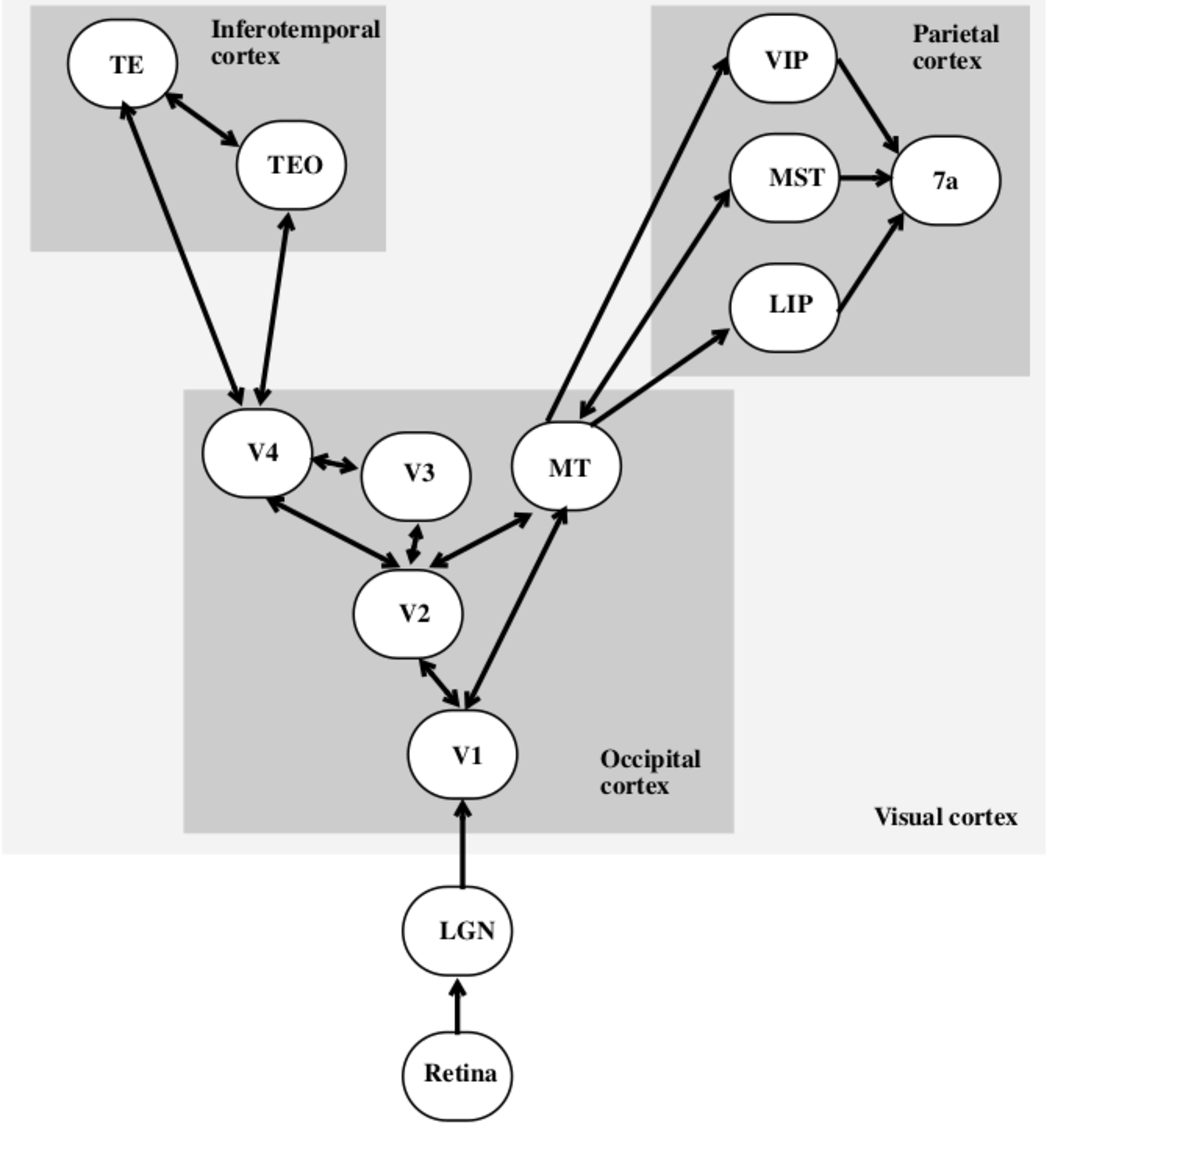
\includegraphics[width=0.8\textwidth]{rolls_pathways.pdf}
%\label{fig:cortex2}
%\end{minipage}
%\caption{carte aplanie des aires du cortex visuel du macaque \cite{primate_cortex_91}, à gauche, et pathways dans ce cortex visuel entre les aires à droite \cite{Rolls2002ComputationalNO}. L'architecture neuronale présente des rétroaction entre zones, dans une architecture non-hiérarchique.}
%\end{figure}
%
% 
%%- Nombreuses études s'appuient sur le système modulaire : le cerveau \cite{primate_cortex_91,mountcastle_columnar_1997,binzegger05}
%%
%%
%%- Modularité hiérarchique( modules de modules) -> Ajouter infos depuis l'article qui parle de modules hiérarchiques. 
%%%Ajouter figure du cerveau avec le schéma des aires
%%
%%Finalement : 
%%Cerveau présente ce qu'on peut appeler des modules, avec des connexions entre eux, avec rétroaction. 
%%
%%Leur mesure peut etre structurelle (regarder les structures de neurones), ou fonctionnelle : quelles aires s'activent pour une fonction ? \\
%%Détail des types de modularité en parties suivantes. 
%
%\subsection{Des réseaux et des modules dans tous les systèmes biologiques}
%
%On a vu dans la partie précédente que les modules sont définis en réponse à un problème de modélisation. Finalement, dans tous les systèmes biolgiques, on peut définir une modularité 
%Pb de modélisation - modularité fonctionnelle
%
%%
%%Les phénomènes émergents ne se limitent pas au cerveau : tous les systèmes biologiques semblent présenter des fonctionnement issus de systèmes complexes, menant à une régulation globale d'une quantité, à un comportement commun, autrement dit, l'émergence d'un comportement. On peut par exemple citer l'exemple des nuées d'oiseaux : des centaines ou des milliers d'oiseaux peuvent voler ensemble, sans se heurter ni se disperser, le tout sans avoir d'instructions globale. Cette capacité à rester en nuée émergent des règles locales que connaissent chacun des oiseaux. Ces règles régissent le comportement individuel à avoir avec leur voisins proches. Ces règles simples permettent à ces milliers d'individus de voler en groupe et de se déplacer.
%%Les arbres en forêt s'adaptent, pour pousser sans se toucher, et partageraient même des information en communiquant. Sans forcément parler d'intelligence, on peut tout à fait voir en ces comportement des mécanismes émergents.
%
%
%%%%%%%%%%%%%%%%%%%%%%%%%%%%%%%%%%%%%%%%%%%%%%%%%%%%%%%%%%%%%%%%%%%%%%%%%%%%%%%%%%%%%%%%%%%%%%%%%%%%%%%%%%%%%%%%%%%%%%%%%%%%%%%%%%%%%%%%%
%% SECTION 3: quel intéret à utiliser des architectures modulaires pour l'apprentissage ? 
%% - 
%%%%%%%%%%%%%%%%%%%%%%%%%%%%%%%%%%%%%%%%%%%%%%%%%%%%%%%%%%%%%%%%%%%%%%%%%%%%%%%%%%%%%%%%%%%%%%%%%%%%%%%%%%%%%%%%%%%%

%\section{Intérêt computationnel des réseaux modulaires, et comment les construire}
%
%Les réseaux modulaires sont ainsi prépondérants dans les systèmes "réels", les systèmes présents dans la nature (réseaux de neurones, biologiques...) ou les réseaux émergents de l'interaction entre humains (réseaux sociaux, réseaux des citations entre auteurs). On retrouve dans tous ces réseaux une structure commune modulaire hiéarchique, parfois avec un aspect invariant d'échelle, les réseaux présentant des hubs. Cette structure de réseau est loin d'un réseau aléatoire et a donc été sélectionné par l'évolution ou les interactions locales. On peut se demander si les réseaux biologiques résultant d'une évolution sélective sont modulaire parce que cette structure présente des avantages computationnels, ou si c'est parce qu'ils résultent d'une évolution sélective modifiant des parties du réseau, qu'ils sont modulaires. 
%Ces avantages motivent l'idée de s'inspirer de réseaux réels pour créer des systèmes computationnels performants et émergents, notamment dans le cadre de l'intelligence artificielle. 
%
%Barabasi : Hypothèse que les réseaux small world présentent un avantage evolutionnaire.
%Modularité hiérarchique présente l'avantage de maintenir une activité dans le réseau sans que ca ne colonise tout ni ne s'eteigne, ce qui est nécessaire pour la computation. 
%
%
%
%\subsection{réponse a un problème de contraintes physiques, énergétiques}
%
%
%- Parallelisme, calcul et small world networks : réponse a un problème de contrainte physiques, énergétiques. 
%- Calcul distribué 
%- Automates cellulaires ?
%
%- Exemple des puces neuromorphiques, calcul embarqué
%
%
%Conclusion: En décentralisant le calcul, on cherche aussi à plus facilement l'utiliser via des architectures neuromorphiques. 
%
%\subsection{Modularité, complexité et émergence d'un apprentissage }
%
%
%Systèmes complexes et emergence: possibilité d'apprentissage, exemple du reservoir computing
%
%La modularité est liée a la complexité des systèmes, donc l'emergence de comportements chaotiques et/ou synchronisés. 
%
%SYSTEMATIC GENERALIZATION : WHAT IS REQUIRED
%AND CAN IT BE LEARNED ? : 
%Our findings show that the generalization of modular models is much more systematic and that it is highly sensitive to the module layout, i.e. to how exactly the modules are connected.
%
%Simplicité de la modularité : exemple de construction des fractales, exemple du rigaudon
%
%Parler des architectures de Hebb (précurseur) ici ou avant ?
%
%slow intermodular processes, fast intramodular : la modularité spatiale a l'origine de différentes échelles temporelles \cite{Pan2009ModularityPS}
%
%
%\subsection{Types de connexions}
%
%Opaque vs tout savoir
%
%
%\subsection{Modularité comme propriété émergente ou modularité définie}
%
%On a défini un réseau modulaire en analysant sa structure ou sa fonction une fois créé. Néanmoins, la façon dont ce réseau a été élaboré peut résulter de plusieurs processus : l'aspect modulaire peut émerger d'une sélection, d'une construction ou d'un recablage des arêtes et des noeuds du graphe; ou alors la modularité peut être définie a priori par la structure du réseau. Cette distinction est nécessaire lorsqu'on cherche à créer des réseaux de neurones pour l'apprentissage, qui sont alors des systèmes qui s'adaptent. La structure peut donc être présente a priori et l'apprentissage uniquement créé par l'adaption de poids au sein du réseau, ou l'apprentissage passe également par l'adaptation des arêtes.
%Au sein même des réseaux dont la structure est définie a priori, la \emph{fonction} de chaque module peut être définie ou non. Dans l'exemple le plus "prédéfini", le réseau d'interaction est défini en liant des modules ayant des fonctions bien précises. C'est le cas par exemple de l'organisation structurelle d'une entreprise, chaque agent ayant un role défini au sein d'une hiérarchie. Ce sont ce genre de modules prédéfinis qui ont été utilisés lors des débuts de la recherche en intelligence artificielle, dans les systèmes experts. Même si ces systèmes ne font pas d'\emph{apprentissage}, un comportement global émerge de l'interaction entre modules. Par exemple, Brooks \cite{brooks_sumsumption_85} propose une architecture en robotique appelée sumsumption, dans laquelle les comportements "intelligents" et haut niveau d'un robot ( "explorer", "planifier") émergent de la combinaison d'actions et de capteurs "bas niveau" comme "tourne", "avance", "faire demi-tour", "detection" (figure~\ref{fig:brooks}).
%
%\begin{figure}
%\centering
%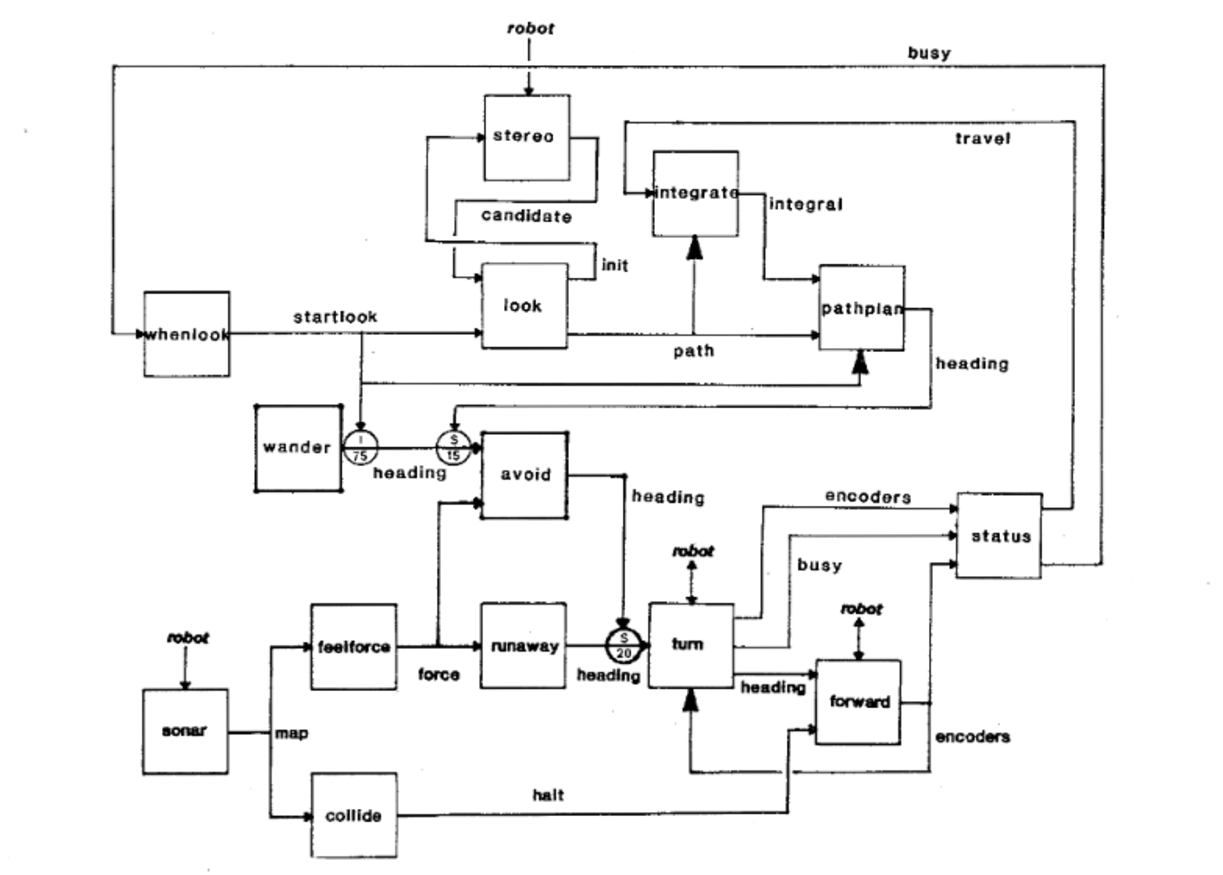
\includegraphics[width=0.5\textwidth]{brooks.pdf}
%\caption{Architecture experte de Brooks. Les modules sont prédéfinis et codent chacun un comportement définis à l'avance. Ils sont connectés en un réseau cablé à l'avance. Cette ingénieurie permet à un robot d'avoir un comportement plus haut niveau que les modules bas niveaux encodés.}
%\label{fig:brooks}
%\end{figure}
%
%Ces réseaux experts précablés ne font pas d'apprentissage. Une main ingénieure doit trouver les bons paramètres, les bonnes connexions, et les bonnes fonctions faisant émerger les comportement voulus. A l'ère de l'apprentissage, on peut remplacer ces modules dont la fonction est prédéfinie par des modules qui apprennent leur fonction. Ils sont alors connectés selon un réseau fixe, mais apprendront au sein de ce réseau leur fonction. 
%
%Enfin, certains réseaux de neurones, bio-inspirés, renforcent une connexion lorsque deux neurones s'activent en même temps. C'est la règle de Hebb "neurones that fire together, wire together". Depuis un bouillon de neurones initial, l'état final du système présente une structure de réseau apprise.  -> Citer des exemples de réseaux qui adaptent des connexions. 
%
%
%Attention : même avec une modularité prédéfinie, on reste un système complexe, donc on pourra avoir des propriétés d'adaptation émergentes.
% 
%%%%%%%%%%%%%%%%%%%%%%%%%%%%%%%%%%%%%%%%%%%%%%%%%%%%%%%%%%%%%%%%%%%%%%%%%%%%
%% SECTION 4 En pratique, ou en est on des réseaux de neurones modulaires ?
%%%%%%%%%%%%%%%%%%%%%%%%%%%%%%%%%%%%%%%%%%%%%%%%%%%%%%%%%%%%%%%%%%%%%%%%%%%%%%ùù
%
%\section{Modularité dans les réseaux de neurones}
%
%Au sein des systèmes complexes, les réseaux de neurones artificiels se sont directement développés en s'inspirant des réseaux biologiques. Hebb formule ainsi en 1949 "neurons that fire together, wire together". Les réseaux de neurones développés depuis sont alors inspirés de la biologie, en s'en éloignant plus ou moins. Quel que soit leur éloignement, ce sont des systèmes complexes dans le sens ou il s'agit d'un grand nombre de neurones reliés entre eux, et qu'on développe dans le but de l'émergence d'une propriété d'apprentissage et de généralisation.
%
%Ces réseaux sont par exemple le perceptron, les cartes auto-organisatrices. 
%L'intérêt de chercher des aspect modulaires des réseaux de neurones a été formulé par exemple par \cite{towards_novel_2001} : 
%
%A partir du perceptron, les réseaux de neurones profond ont été développés comme une assemblée de perceptrons reliés hiérachiquement (fin 90 ) 
%
%\subsection{Deep Learning}
%Boites noires qui ont des performances remarquables sur tous les domaines, leur représentation et compréhension est quant à elle toujours un challenge. Ajouter un aspect modulaire non-hiérarchique dans les calculs de ce genre de réseau, pour augmenter la vitesse d'apprentissage ou encore pour 
%
%\subsubsection{Réseaux de neurones profond et modulaires}
%
%- Réseaux qui apprennent a s'organiser en modules. Interet. Limites ? Performances ? \cite{Andreas2016NeuralMN,Kirsch2018ModularNL}
%"The NMN approach is intuitively appealing but its
%widespread adoption has been hindered by the large amount of domain knowledge that is required
%to decide (Andreas et al., 2016) or predict (Johnson et al., 2017; Hu et al., 2017) how the modules
%should be created (parametrization) and how they should be connected (layout) based on a natural
%language utterance. Besides, their performance has often been matched by more traditional neural
%models" ( systematic generalization article ) 
%
%\subsubsection{Utiliser des modules pour mieux représenter les réseaux de neurones profond}
%
%
%- Trouver des modules dans les réseaux pour les expliquer ? \cite{Watanabe2018ModularRO,Csordas2021AreNN}
%are neural net modular : "it uses different modules for very different functions = Pspecialize," et "it uses the same module for identical functions that
%may have to be performed multiple times = Preuse"
%- Reconciling deep learning with symbolic artificial intelligence: representing objects and relations(2019)
%Pb du deep learning = Data inefficiency (comparé a l'humain);Poor generalisation; Lack of interpretability.
%
%\subsection{Réseaux auto-organisés}
%
%Les réseaux auto-organisés sont directement inspirés des réseaux biologiques. Au sein de ces réseaux
%Plus qu'en deep learning, les réseaux de neurones auto-organisés
%- Auto-organisation prend une profonde inspiration biologique, tout comme les modules.
%- Exemple de réseaux auto-organisés modulaires : développer dans la partie suivante.
%\begin{figure}
%\begin{minipage}{0.5\textwidth}
%
%%\centering
%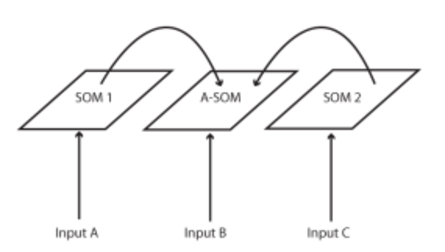
\includegraphics[width=\textwidth]{asom}
%\caption{A-SOM model \cite{johnsson_associative_2009}}
%\end{minipage}
%\begin{minipage}{0.5\textwidth}
%%\centering
%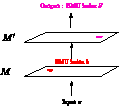
\includegraphics[width=0.9\textwidth]{hsom}
%\caption{HSOM model \cite{LampinenClusteringPO}}
%
%\end{minipage}
%\end{figure}
%\cite{LampinenClusteringPO}
%
%\cite{parisiLL}
%
%Lefort
%
%Travaux préliminaires de l'équipe ->  Bassem, Ménard ?
%
%
%
%\subsection{Construire une architecture modulaire}
%
%A mettre dedans : 
%
%- Réseaux top down / modulaires ? définition, a quel point un réseau est modulaire, qu'est ce qu'on appelle réseau modulaire ? 
%Fonction définies au préalable vs émergence des fonctions. 
%Modules définis au préalable vs émergence des modules. 
%
%
%%%%%%%%%%%%%%%%%%%%%%%%%%%%%%%%%%%%%%%%%%%%%%%%%%%%%%%%%%%%%%%%%%%%%%%%%%%%%%%%%
%% SECTION 5 : proposer des enjeux par rapports au réseaux listés précedemment 
%%%%%%%%%%%%%%%%%%%%%%%%%%%%%%%%%%%%%%%%%%%%%%%%%%%%%%%%%%%%%%%%%%%%%%%%%%%%%%%%%
%
%
%\section{Enjeux d'une architecture modulaire de SOMs}
%
%On connait plutot bien les SOM, mais on sait que des comportements nouveaux peuvent émerger lorsqu'on met en interaction des systèmes étudiés séparément. 
%On peut donc se poser la question des comportements qui peuvent survenir dans ce cas.
%
%Dans les structures de cartes étudiés, modularité forte dans le sens ou les fonctions des modules sont prédéfinies. Si on ne fournit que les règles d"interaction, ou est ce qu'on se situe ? 
% 
% 
%Position du manuscrit : architecture 
%%%%%%%%%%%%%%%%%%%%%%%%%%%%%%%%%%%%%%%%%
%
%Plan de la partie ! 
%
% 
%
%\begin{enumerate}
%\item Intro : Notre monde est modulaire, en tout cas nous l'interprétons en tant que tel. Proposé déjà dans les années 60 - breve histoire des réseaux de neurones ?
%Remarquer que nous, observeur, raisonne et se construit modualairement. Il nous est difficile de concevoir les choses autrement. 
%Les disciplines sientifiques par ex, un domaine obéit a des principes
%\item Qu'appelle t-on la modularité ? Définitions claires et propriétés
%	\begin{itemize}
%
%		\item Definition
%			\begin{enumerate}
%			\item Structurelle, dans les systèmes réseaux
%			\item Fonctionnelle, dans les systèmes dont on ne connait pas la structure ?\\
%			\item Temporelle / mais est ce que le temps ce n'est qu'une dim de plus
%			\item Modularité hiérarchique attention : deux defs a hiérarchiques. Soit c'est une histoire de connexions, soit d'auto-similarité. On parle nous de l'auto similarité !!! Au contraire l'autre forme de hiérarchie n'est pas observée en bio.
%			\end{enumerate}
%		
%		\item Propriétés de la modularité 
%			\begin{enumerate}
%			\item Auto-organisation
%			\item Types de connexions
%			\item Emergence
%			\end{enumerate}
%	\end{itemize}	
%\item Exemples Biologiques et computationnels
%	\begin{enumerate}
%	\item Biologie : opti evolution a priori...
%	\item Computationnel : pareil.
%	\end{enumerate}
%	
%\item Maintenant qu'on sait ce que sont les systèmes modulaires, en quoi on peut faire de l'apprentissage avec ? Quels sont les intérêts ?
%	\begin{enumerate}
%		\item Exemples de réseaux auto-organisés
%		\item Exemples de réseaux de neurones : deep learning
%	\end{enumerate}
%
%\end{enumerate}





